\documentclass{beamer}
\usepackage{amsmath}
\usepackage{apacite}
\usepackage{caption}
\usepackage[font=small, labelfont=bf]{subcaption}
\usepackage{textpos}
\usetheme{Darmstadt}
\usepackage{graphicx}
\usepackage{float}
%packages for definitions%%%%%%%%%%%%%%
\usepackage{blindtext}
\usepackage{scrextend}
\usepackage{amsmath}
\addtokomafont{labelinglabel}{\sffamily}
\usepackage{tikz}
    \usetikzlibrary{shapes}
    \usetikzlibrary{positioning}
    \usetikzlibrary{arrows}
    \usetikzlibrary{fit}
    \usetikzlibrary{decorations.pathreplacing}
    \usetikzlibrary{shadows.blur}
    \usetikzlibrary{shapes.symbols}

% Remove the useless and unsightly black bar at the top of the slides
\setbeamertemplate{headline}{}
% Remove the navigation thing at the bottom of the slides.
\setbeamertemplate{navigation symbols}{}

% Colors for Auburn University from their marketing materials
% http://www.ocm.auburn.edu/graphicservices/colors.html
\definecolor{auburn_orange}{RGB}{232, 119, 34}
\definecolor{auburn_blue}{RGB}{12, 35, 64}
% Set the color of the slide headers to auburn blue
\setbeamercolor{structure}{fg=auburn_blue}

% a new command for a four quadrant slide mardas
\newcommand\FourQuad[4]{%
    \begin{minipage}[b][.35\textheight][t]{.47\textwidth}#1\end{minipage}\hfill%
    \begin{minipage}[b][.35\textheight][t]{.47\textwidth}#2\end{minipage}\\[0.5em]
    \begin{minipage}[b][.35\textheight][t]{.47\textwidth}#3\end{minipage}\hfill
    \begin{minipage}[b][.35\textheight][t]{.47\textwidth}#4\end{minipage}%
}

%%%%%%%%%%%%%%%%%%%%%%%%%%%%%%%%%%%%%%%
\AtBeginSection[]{
    \begin{frame}
    \vfill
    \centering
    \begin{beamercolorbox}[sep=8pt,center,shadow=true,rounded=true]{title}
        \usebeamerfont{title}\insertsectionhead\par%
    \end{beamercolorbox}
    \vfill
    \end{frame}
}

\title{A Neural Algorithm of Artistic Style \\ { \tiny \citeA{gatys2016image}}}
\author{Behnam Rasoolian, Christian Kauten}
\institute{Auburn University}
\date{}

\begin{document}
\tikzset{
    mystyle/.style={
    inner sep=0pt,
    minimum width = .5cm,
    minimum height = .5cm,
    text width=1cm,
    circle,
    draw=black,
    align=center,
  }
}
\tikzset{
    myEdgeStyle/.style={
    ->,
    line width = 1pt
    %ultra thick
  }
}
\tikzset{
    myArrow/.style={
    single arrow,
    draw,
    text width =.3cm,
    scale=.8,
    shade, shading=axis, left color=orange, right color=yellow,
        shading angle=45,
    blur shadow={shadow blur steps=5,shadow blur extra rounding=1.3pt}
}
}



\frame{\titlepage}



\begin{frame}{Introduction}
    \begin{itemize}
    \item[] It is a variation of texture transfer problem:\\
    Given a source image, synthesize a new texture which preserves the
    semantic content of the original image.
    \item[] \textbf{Input:}
        \begin{itemize}
            \item An input image that represents the content
            \item A work of art that represents the style
        \end{itemize}
    \item[] \textbf{Output:}
        \begin{itemize}
            \item A new image that is perceptually similar in style to
            the work of art and in content to the original image.
        \end{itemize}
    \end{itemize}
\end{frame}



\begin{frame}{Introduction}
\begin{figure}[ht]
\centering
\includegraphics[width=\textwidth]{img/content/samford-sign}
\caption*{\textbf{Content Image:} Samford Hall, Auburn, AL}
\end{figure}
\end{frame}



\begin{frame}{Introduction}
\begin{figure}[ht]
\centering
\includegraphics[height=0.7\textheight]{img/artworks/seated-nude}
\caption*{\textbf{Artwork Image:} Pablo Picasso's \textit{Seated Nude}}
\end{figure}
\end{frame}



\begin{frame}{Introduction}
\begin{figure}[ht]
\centering
\includegraphics[width=\textwidth]{img/loss/Adam.png}
\caption*{\textbf{Output Image:} Samford Hall Styled like \textit{Seated Nude}}
\end{figure}
\end{frame}



\begin{frame}{Approach in this paper}
    \begin{enumerate}
        \item Pick a CNN architecture trained for a classification task
        \begin{itemize}
            \item in this case we use \textbf{VGG19} trained on
                \textbf{ImageNet}
        \end{itemize}
        \item Design a loss function that balances content of an image with
            styles and textures from a work of art
        \item Optimize a white noise image based on this loss function to
            capture both content of the image and style of the work of art.
    \end{enumerate}
\end{frame}



\begin{frame}{Approach in this paper}
\framesubtitle{VGG19}
\begin{figure}[H]
\centering
\includegraphics[width=\textwidth]{img/vgg19/classification}
\caption*{VGG19 Image Classification Architecture}
\end{figure}
\end{frame}



\begin{frame}{Approach in this paper}
\framesubtitle{VGG19}
\begin{figure}[H]
\centering
\includegraphics[width=.9\textwidth]{img/vgg19/feature-extraction}
\caption*{VGG19 Image Feature Extraction Architecture}
\end{figure}
\end{frame}



\begin{frame}{Approach in this paper}
\framesubtitle{VGG19}
\begin{figure}[H]
\centering
\includegraphics[width=.9\textwidth]{img/vgg19/synthesis}
\caption*{VGG19 Image Synthesis Architecture \cite{gatys2016image}}
\end{figure}
\end{frame}



\begin{frame}{Approach in this paper}
    \framesubtitle{Loss function}

    Two different loss functions are taken into account:

    \begin{enumerate}
        \item $\mathcal{L}_{content}$ captures the difference in content
            between two images by measuring the distance between features at
            each level.
        \item $\mathcal{L}_{style}$ captures the the difference in style
            between two images by evaluating the distance between the two
            \textbf{Gram Matrices} at each level.
    \end{enumerate}

    The total loss function is a
    \textbf{\color{red} linear combination}
    of the content and style losses:

    \begin{equation}
    \mathcal{L}_{total} =
    \alpha \mathcal{L}_{content} +
    \beta \mathcal{L}_{style}
    \end{equation}
\end{frame}



% Gatys et al. visualize of network passes
\begin{frame}{Approach in this paper}
\framesubtitle{Architecture}
\begin{figure}[ht]
\centering
\caption*{Style Transfer Architecture}
\includegraphics[width=\textwidth]{img/style-transfer}
\end{figure}
\end{frame}



\begin{frame}{Notations}
    \begin{itemize}
        \item $\mathbf{P}$: The original, content image
        \item $\mathbf{A}$: The original, artwork image
        \item $\mathbf{X}$: The image to be generated. It is initiated as a
            random noise image.
        \item $F^l$: \textbf{Feature Map} or \textbf{Activation Map}
            at level l, is the result of applying
            filters at level $l$. If $N_l$ filters are applier at level $l$,
            then this feature map has a depth of $N_l$.
        \item $N_l$: The number of filters applier at level $l$. This is
            the same as the depths of the feature map at level
            $l$.
        \item $M_l$: the dimension of the feature map at level l, which
            is equal to $w_l \times h_l$.
        \item The feature map is $M_l \times N_l$.
    \end{itemize}
\end{frame}



\begin{frame}{Notations}
    \begin{figure}[H]
        \centering
        \includegraphics[width=.8\textwidth]{img/levels}
    \end{figure}
\end{frame}



\begin{frame}{Content Representation}
    \begin{itemize}
        \item Perform gradient descent optimization on a white noise image
            ($\mathbf{X}$) and a content image ($\mathbf{P}$)
        \item $F_X^l$ and $F_P^l$: Respective feature maps of the noise image
            and the original image
        \item Goal: Reduce the squared-error loss between $F^l$ and $P^l$.
    \begin{equation}
        \mathcal{L}_{content}(\mathbf{P}, \mathbf{X}, l) =
        \frac{1}{2} \sum_{i=1}^{N_l}\sum_{j=1}^{M_l}{((F_X)^l_{ij} - (F_P)^l_{ij})^2}
    \end{equation}
    \end{itemize}
\end{frame}



\begin{frame}{Content Representation}
    The gradient of this loss with respect to activations in $l$ can be easily
    calculated:
    \begin{equation}
        \frac{\partial \mathcal{L}_{content}}{\partial F^l_{ij}}
        =
        \begin{cases}
            (F^l_x - F^l_p)_{ij} & \iff (F^l_X)_{ij} > 0 \\
            0 & \iff (F^l_X)_{ij} < 0 \\
        \end{cases}
    \end{equation}
\end{frame}



\begin{frame}{Content Reconstruction}
\begin{figure}[ht]
    \begin{minipage}[b]{0.45\linewidth}
        \centering
        \includegraphics[width=\textwidth]{img/content/noise}
        \caption*{White Noise Image $\mathbf{x}$}
    \end{minipage}
    \hspace{0.5cm}
    \begin{minipage}[b]{0.45\linewidth}
        \centering
        \includegraphics[width=\textwidth]{img/content/tubingen}
        \caption*{Content Image $\mathbf{p}$}
    \end{minipage}
\end{figure}
\end{frame}



% 1:1
\begin{frame}{Content Reconstruction}
\begin{figure}[ht]
\centering
\includegraphics[width=0.8\textwidth]{img/vgg19/content/block1_conv1}
\caption*{Block 1 Conv 1}
\end{figure}
\end{frame}



\begin{frame}{Content Reconstruction}
\begin{figure}[ht]
\centering
\includegraphics[width=.8\textwidth]{img/content/block1_conv1}
\caption*{Block 1 Conv 1}
\end{figure}
\end{frame}



% 2:1
\begin{frame}{Content Reconstruction}
\begin{figure}[ht]
\centering
\includegraphics[width=0.8\textwidth]{img/vgg19/content/block2_conv1}
\caption*{Block 2 Conv 1}
\end{figure}
\end{frame}
\begin{frame}{Content Reconstruction}
\begin{figure}[ht]
\centering
\includegraphics[width=.8\textwidth]{img/content/block2_conv1}
\caption*{Block 2 Conv 1}
\end{figure}
\end{frame}



% 3:1
\begin{frame}{Content Reconstruction}
\begin{figure}[ht]
\centering
\includegraphics[width=0.8\textwidth]{img/vgg19/content/block3_conv1}
\caption*{Block 3 Conv 1}
\end{figure}
\end{frame}
\begin{frame}{Content Reconstruction}
\begin{figure}[ht]
\centering
\includegraphics[width=.8\textwidth]{img/content/block3_conv1}
\caption*{Block 3 Conv 1}
\end{figure}
\end{frame}



% 4:1
\begin{frame}{Content Reconstruction}
\begin{figure}[ht]
\centering
\includegraphics[width=0.8\textwidth]{img/vgg19/content/block4_conv1}
\caption*{Block 4 Conv 1}
\end{figure}
\end{frame}
\begin{frame}{Content Reconstruction}
\begin{figure}[ht]
\centering
\includegraphics[width=.8\textwidth]{img/content/block4_conv1}
\caption*{Block 4 Conv 1}
\end{figure}
\end{frame}



% 5:1
\begin{frame}{Content Reconstruction}
\begin{figure}[ht]
\centering
\includegraphics[width=0.8\textwidth]{img/vgg19/content/block5_conv1}
\caption*{Block 5 Conv 1}
\end{figure}
\end{frame}
\begin{frame}{Content Reconstruction}
\begin{figure}[ht]
\centering
\includegraphics[width=.8\textwidth]{img/content/block5_conv1}
\caption*{Block 5 Conv 1}
\end{figure}
\end{frame}




\begin{frame}{Style Representation}
Style representation is achieved via the ``Gram Matrix'' $G$. Gram matrix is
an $N_l \times N_l$ matrix which calculates the correlations between
different filter responses.

\begin{equation}
    \mathbf{G^l}_{ij} = \mathbf{{F^l}^T}_i \times \mathbf{F^l}_j
    = (\mathbf{{F^l}^T} \times \mathbf{F^l})_{ij}
\end{equation}
\end{frame}



\begin{frame}{Style Representation}
Given $G_x^l$ and $G_a^l$ as respective Gram matrices of the noise image and
the original image, our goal is to reduce the overall difference between
$G_x^l$ and $G_a^l$. In this sense, Contribution of layer $l$ to the total
loss is

\begin{equation}
    E_l = \frac{1}{4N_l^2M_l^2} \sum_{i}^{N_l}\sum_{j}^{N_l}{((G^l_x)_{ij} - (G_a^l)_{ij})^2}
    = \mathbf{1}^T(\mathbf{G^l_x} - \mathbf{G^l_a})(\mathbf{G^l_x} - \mathbf{G^l_a})^T
\end{equation}

\end{frame}



\begin{frame}{Style Representation}
The total style loss is:
\begin{equation}
    \mathcal{L}_{style}(\mathbf{a}, \mathbf{x}) = \sum_{l=0}^L {w_l E_l }
\end{equation}
\begin{equation}
    \frac{\partial \mathcal{L}_{style}}{\partial (F_x^l)_{ij}} = \frac{\partial E_l}{\partial (F^l_x)_{ij}} =
    (4(\mathbf{G_x}^l - \mathbf{G_a}^l) \times \mathbf{F_x}^l)_{ij}
\end{equation}
\end{frame}



\begin{frame}{Style Representation}
\begin{equation}
    \frac{\partial \mathcal{L}_{style}}{\partial (F^l_x)_{ij}} = \frac{\partial E_l}{\partial (F^l_x)_{ij}} =
    (4(\mathbf{G_x}^l - \mathbf{G_a}^l) \times \mathbf{F}_x^l)_{ij}
\end{equation}
    \begin{figure}
    \begin{tikzpicture}[scale=.84, every node/.style={scale=.7}, transform shape]
        \node (a) at (-5, 0) {};
        \node [mystyle] (b) [right=2cm of a] {$ \times X^T$};
        \draw [myEdgeStyle] (a.east) to  node [auto] (ab) {$\mathbf{F^l}_{N_l \times M_l}$}(b.west);
        \draw [myEdgeStyle] (a.east) to  node [red] [below] (ab) {$2(\mathbf{G_x} - \mathbf{G_a}) \times 2\mathbf{F}$}(b.west);
        \node [mystyle, ellipse, text height = .5cm, text width = 2cm] (c) [right=2cm of b] {$ (\mathbf{X} - \mathbf{G_a}_l)^2$};
        \draw [myEdgeStyle] (b.east) to node [auto] (bc) {$\mathbf{G_x}_{N_l \times N_l}$} (c.west) ;
        \draw [myEdgeStyle] (b.east) to node  [red][below] (bc) {$2(\mathbf{G_x} - \mathbf{G_a})_{N_l \times N_l}$} (c.west) ;
        \node [mystyle] (d) [right=2cm of c] {$\times$};
        \draw [myEdgeStyle] (c.east) to node [auto] (cd) {$(G_x - G_a)^2_{N_l \times N_l}$} (d.west) ;
        \draw [myEdgeStyle] (c.east) to node  [red][below] (cd) {$1_{N_l \times N_l}$} (d.west) ;
        \node (bcd) [below=1cm of cd] {};
        \draw [myEdgeStyle] (bcd.east) -| node [above left= .1and .4cm] {$\mathbf{1}_{N_l \times 1}$} (d.south) ;
        \node [mystyle] (e) [right=2cm of d] {$\times$};
        \draw [myEdgeStyle] (d.east) to node [above] (de) {$E'_{N_l \times 1}$} (e.west) ;
        \draw [myEdgeStyle] (d.east) to node  [red][below] (de) {$\mathbf{1}_{N_l \times 1}$} (e.west) ;
        \node (bde) [below=1cm of de] {};
        \draw [myEdgeStyle] (bde.east) -| node [above left= .1and .4cm] {$\mathbf{1}^T_{1 \times N_l}$} (e.south) ;
        \node (f) [right=1.5cm of e] {};
        \draw [myEdgeStyle] (e.east) to node [auto] (ef) {$E$} (f.west) ;
        \draw [myEdgeStyle] (e.east) to node  [red][below] (ef2) {$1$} (f.west) ;
    \end{tikzpicture}
    \end{figure}
\end{frame}



\begin{frame}{Style Reconstruction}
\begin{figure}[ht]
    \begin{minipage}[b]{0.45\linewidth}
        \centering
        \includegraphics[width=\textwidth]{img/style/noise}
        \caption*{White Noise Image $\mathbf{x}$}
    \end{minipage}
    \hspace{0.5cm}
    \begin{minipage}[b]{0.45\linewidth}
        \centering
        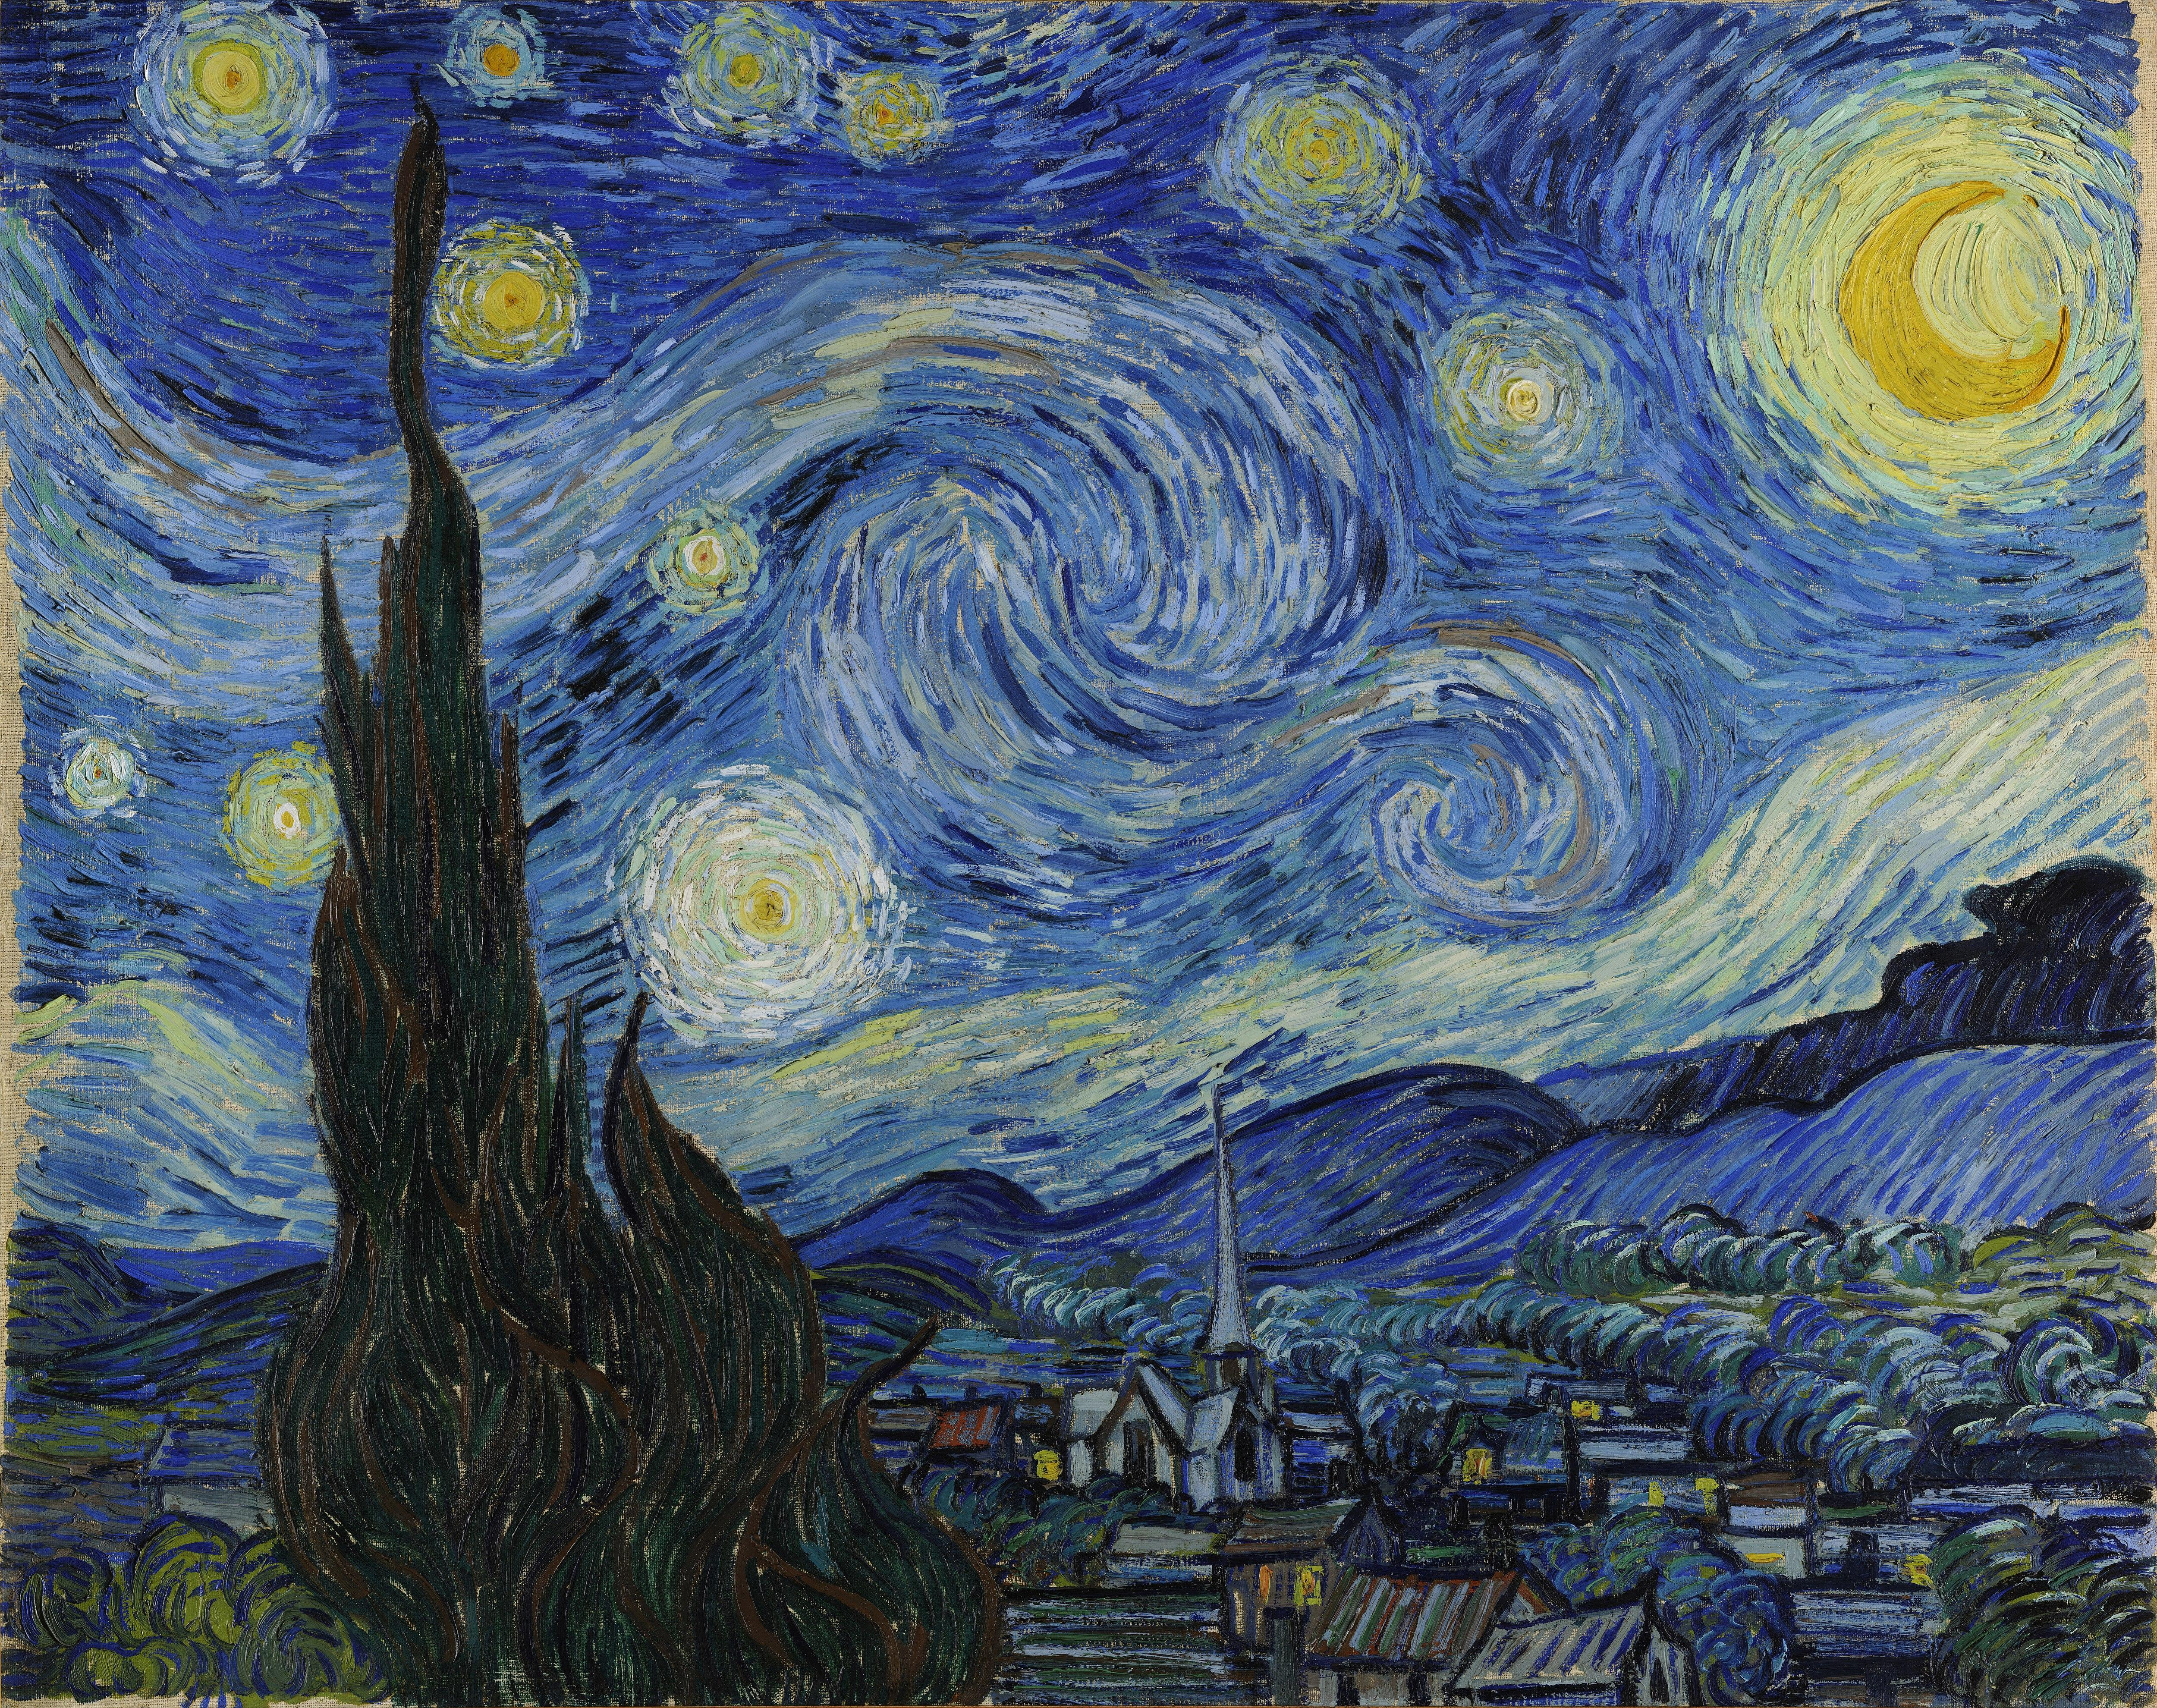
\includegraphics[width=\textwidth]{img/style/the-starry-night}
        \caption*{Artwork Image $\mathbf{a}$}
    \end{minipage}
\end{figure}
\end{frame}



% 1:1
\begin{frame}{Style Reconstruction}
\begin{figure}[ht]
\centering
\includegraphics[width=0.9\textwidth]{img/vgg19/style/block1_conv1}
\caption*{Conv 1 of Block 1}
\end{figure}
\end{frame}
\begin{frame}{Style Reconstruction}
\begin{figure}[ht]
\centering
\includegraphics[width=.8\textwidth]{img/style/block1_conv1}
\caption*{Conv 1 of Block 1}
\end{figure}
\end{frame}



% [1,2]:1
\begin{frame}{Style Reconstruction}
\begin{figure}[ht]
\centering
\includegraphics[width=0.8\textwidth]{img/vgg19/style/block2_conv1}
\caption*{Conv 1 of Block 1, 2}
\end{figure}
\end{frame}
\begin{frame}{Style Reconstruction}
\begin{figure}[ht]
\centering
\includegraphics[width=.8\textwidth]{img/style/block2_conv1}
\caption*{Conv 1 of Block 1, 2}
\end{figure}
\end{frame}



% [1,2,3]:1
\begin{frame}{Style Reconstruction}
\begin{figure}[ht]
\centering
\includegraphics[width=0.9\textwidth]{img/vgg19/style/block3_conv1}
\caption*{Conv 1 of Block 1, 2, 3}
\end{figure}
\end{frame}
\begin{frame}{Style Reconstruction}
\begin{figure}[ht]
\centering
\includegraphics[width=.8\textwidth]{img/style/block3_conv1}
\caption*{Conv 1 of Block 1, 2, 3}
\end{figure}
\end{frame}



% [1,2,3,4]:1
\begin{frame}{Style Reconstruction}
\begin{figure}[ht]
\centering
\includegraphics[width=0.8\textwidth]{img/vgg19/style/block4_conv1}
\caption*{Conv 1 of Block 1, 2, 3, 4}
\end{figure}
\end{frame}
\begin{frame}{Style Reconstruction}
\begin{figure}[ht]
\centering
\includegraphics[width=.8\textwidth]{img/style/block4_conv1}
\caption*{Conv 1 of Block 1, 2, 3, 4}
\end{figure}
\end{frame}



% [1,2,3,4,5]:1
\begin{frame}{Style Reconstruction}
\begin{figure}[ht]
\centering
\includegraphics[width=0.8\textwidth]{img/vgg19/style/block5_conv1}
\caption*{Conv 1 of Block 1, 2, 3, 4, 5}
\end{figure}
\end{frame}
\begin{frame}{Style Reconstruction}
\begin{figure}[ht]
\centering
\includegraphics[width=.8\textwidth]{img/style/block5_conv1}
\caption*{Conv 1 of Block 1, 2, 3, 4, 5}
\end{figure}
\end{frame}



% Style transfer loss (total loss)
\begin{frame}{Style Transfer}
To transfer the style of an artwork $\textbf{a}$, onto some content image
$\textbf{P}$, we form the joint loss function of $L_{content}$ and
$L_{style}$:

\begin{equation}
    \mathcal{L}_{total}(\mathbf{P}, \mathbf{a}, \mathbf{x}) =
    \alpha \mathcal{L}_{content}(\mathbf{P}, \mathbf{x}) +
    \beta \mathcal{L}_{style}(\mathbf{a}, \mathbf{x})
\end{equation}

where $\alpha$ and $\beta$ are the arbitrary weighting factors of the content
and style loss respectively. Gatys et al. find the best results using a ratio
of $\alpha, \beta \in [5\times10^{-4}, 5\times10^{-3}]$.
\end{frame}



% white noise and style representation
\begin{frame}{Style Transfer}
\begin{figure}[ht]
    \begin{minipage}[b]{0.34\linewidth}
        \centering
        \includegraphics[width=\textwidth]{img/content/tubingen}
        \caption*{content image $\mathbf{p}$}
    \end{minipage}
    \hspace{0.5cm}
    \begin{minipage}[b]{0.34\linewidth}
        \centering
        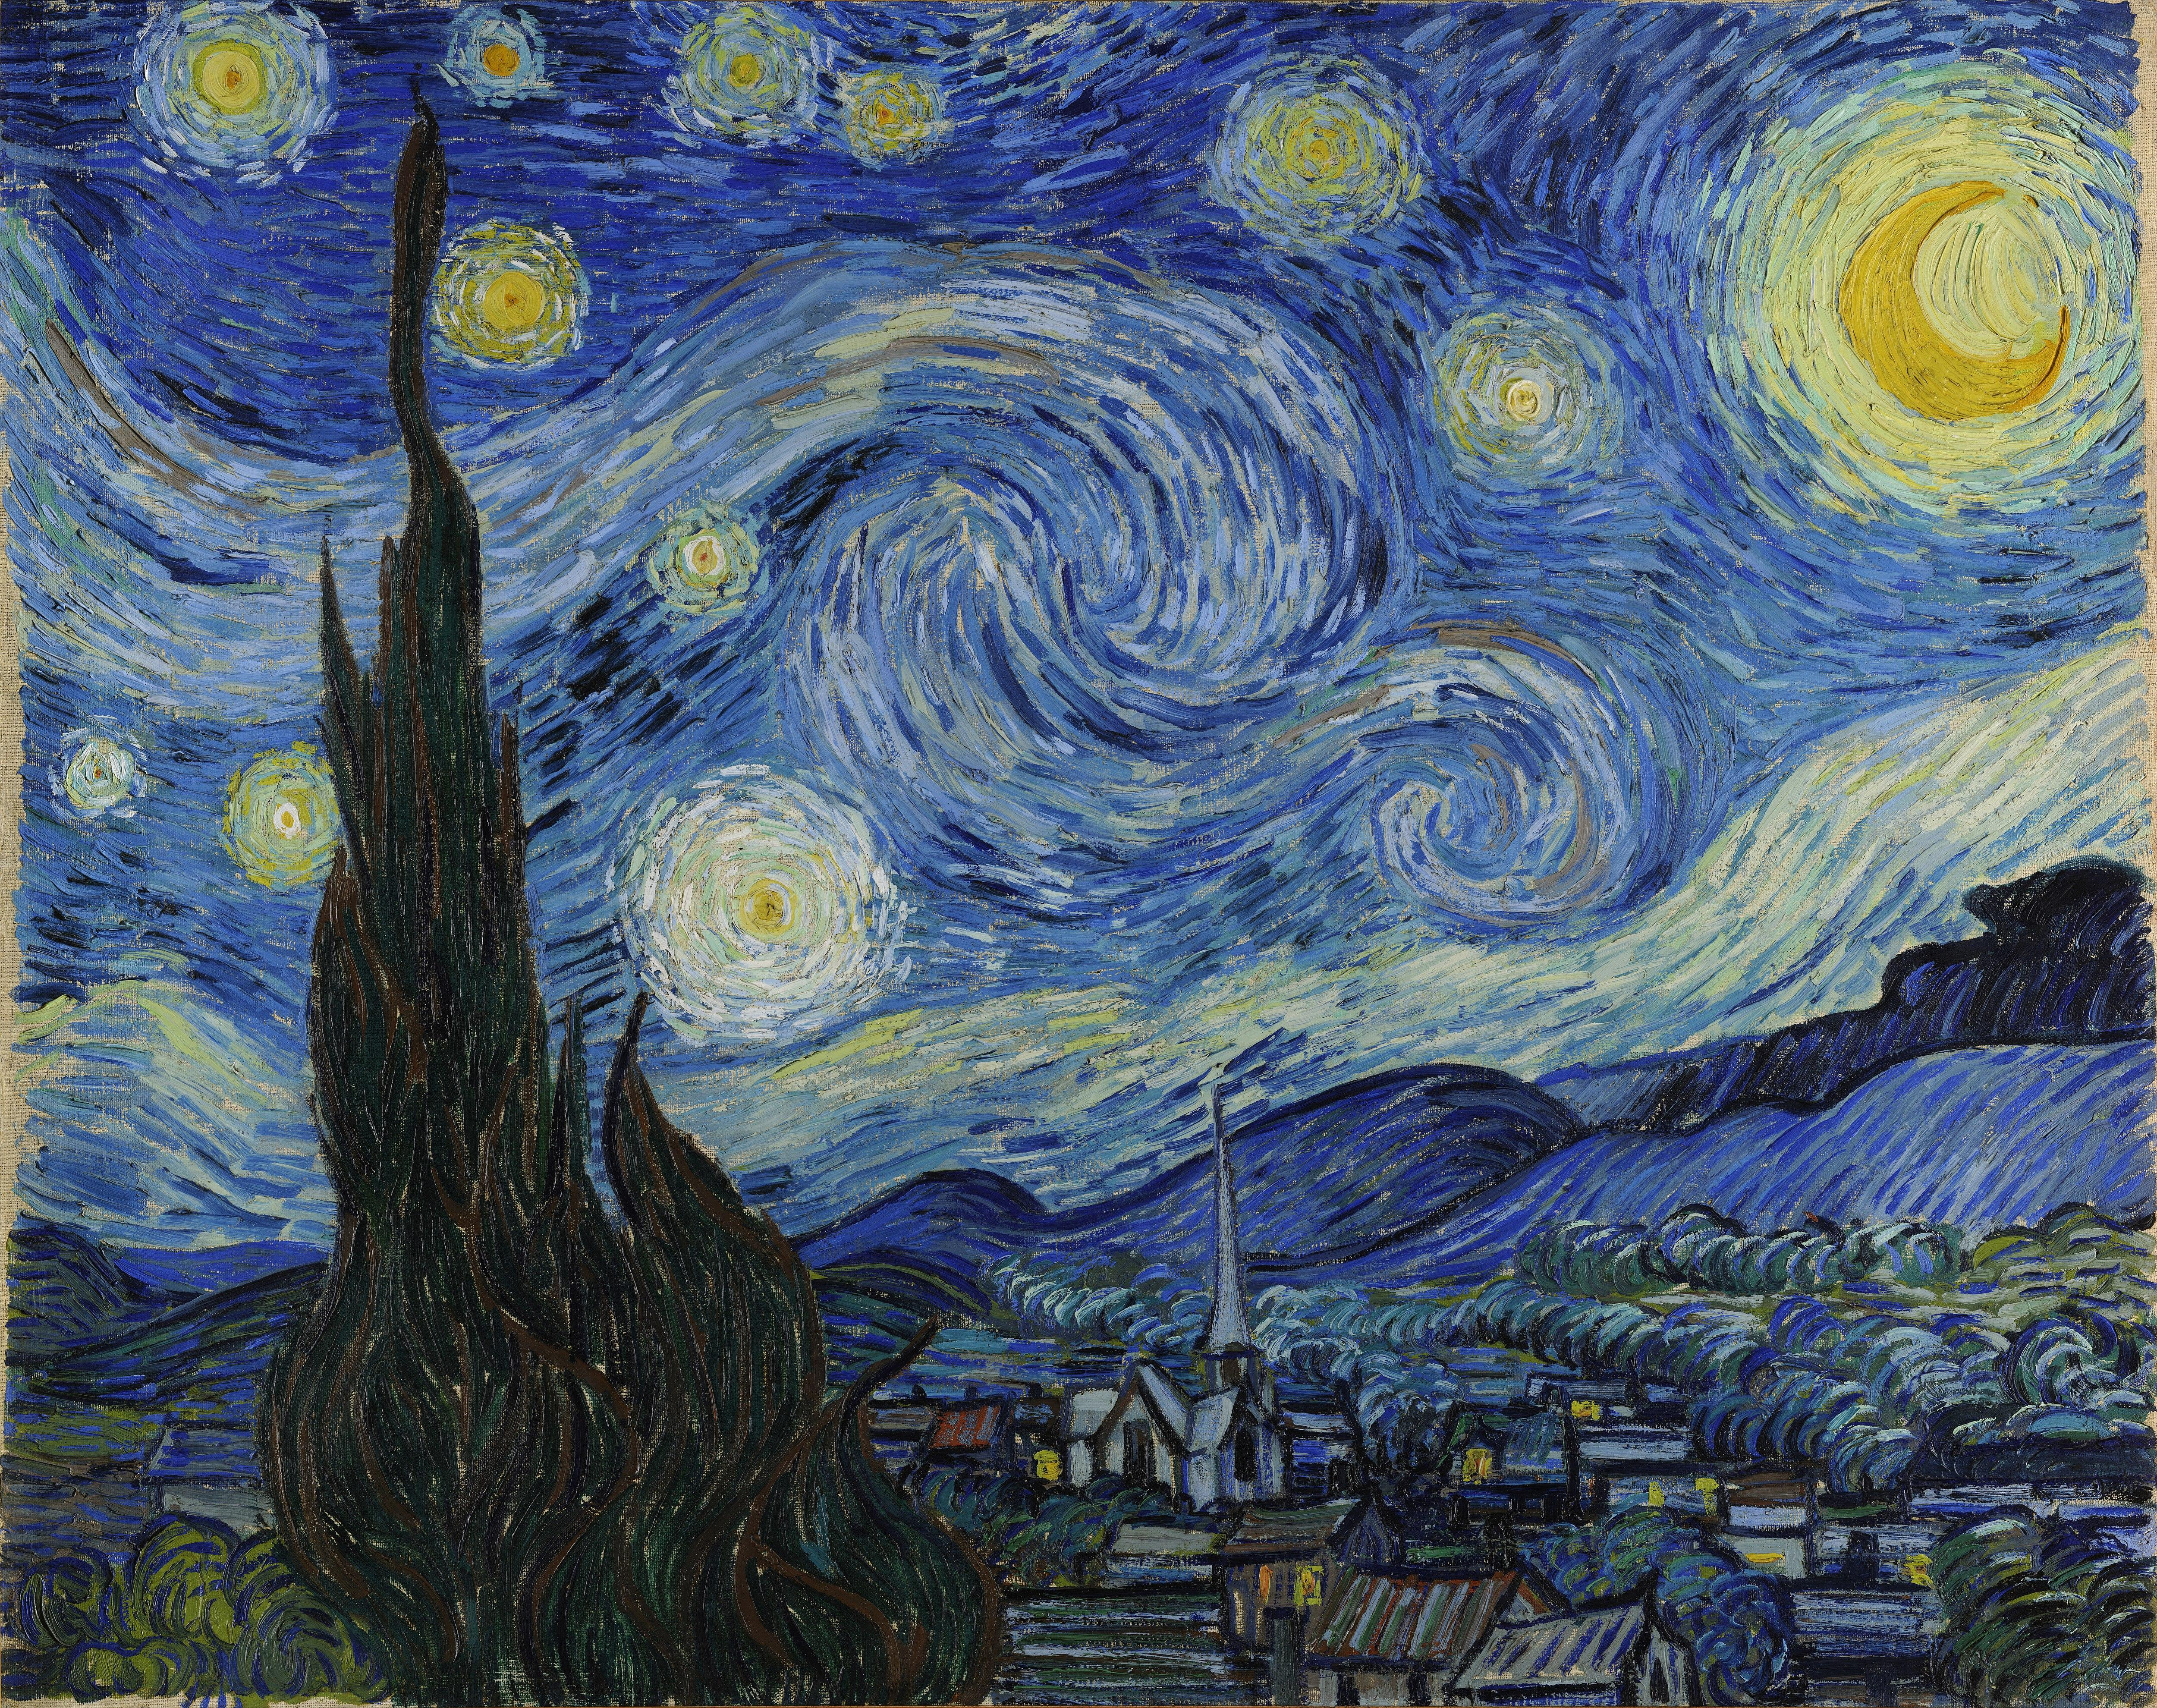
\includegraphics[width=\textwidth]{img/style/the-starry-night}
        \caption*{artwork image $\mathbf{a}$}
    \end{minipage}
    \hspace{0.5cm}
    \begin{minipage}[b]{0.34\linewidth}
        \centering
        \includegraphics[width=\textwidth]{img/style/noise}
        \caption*{white noise image $\mathbf{x}$}
    \end{minipage}
\end{figure}
\end{frame}



% VGG19 for style transfer
\begin{frame}{Style Transfer}
\begin{figure}[ht]
\centering
\caption*{Content and Style Loss Layers for Style Transfer}
\includegraphics[width=0.9\textwidth]{img/vgg19/transfer/layers}
\end{figure}
\end{frame}



% Gatys et al. visualize of network passes
\begin{frame}{Style Transfer}
\begin{figure}[ht]
\centering
\caption*{Style Transfer Architecture}
\includegraphics[width=\textwidth]{img/style-transfer}
\end{figure}
\end{frame}



% picture of Tubingen, the content image p
\begin{frame}{Style Transfer}
\begin{figure}[H]
\centering
\includegraphics[width=.8\textwidth]{img/content/tubingen}
\caption*{Content Image \textbf{p}, Tubingen Germany}
\end{figure}
\end{frame}



% 4 pane with the 4 Artworks for stylization
\begin{frame}{Style Transfer}
\begin{figure}
\centering
\FourQuad{
    \begin{figure}[ht]
    \centering
    \caption*{The Shipwreck of the Minotaur}
    \includegraphics[width=0.8\textwidth,height=0.27\textheight]{img/artworks/the-shipwreck-of-the-minotaur}
    \end{figure}
}{
\vfill
    \begin{figure}[ht]
    \centering
    \caption*{The Starry Night}
    \includegraphics[width=0.8\textwidth,height=0.27\textheight]{img/artworks/the-starry-night}
    \end{figure}
}{
    \begin{figure}[ht]
    \centering
    \caption*{Seated Nude}
    \includegraphics[width=0.8\textwidth,height=0.27\textheight]{img/artworks/seated-nude}
    \end{figure}
}{
    \begin{figure}[ht]
    \centering
    \caption*{The Scream}
    \includegraphics[width=0.8\textwidth,height=0.27\textheight]{img/artworks/the-scream}
    \end{figure}
}
\caption*{Artwork Image \textbf{a}}
\end{figure}
\end{frame}



% 4 pane with the 4 stylized artworks
\begin{frame}{Style Transfer}
\begin{figure}
\centering
\FourQuad{
    \begin{figure}[ht]
    \centering
    \caption*{The Shipwreck of the Minotaur}
    \includegraphics[width=0.8\textwidth,height=0.27\textheight]{img/transfer/the-shipwreck-of-the-minotaur}
    \end{figure}
}{
\vfill
    \begin{figure}[ht]
    \centering
    \caption*{The Starry Night}
    \includegraphics[width=0.8\textwidth,height=0.27\textheight]{img/transfer/the-starry-night}
    \end{figure}
}{
    \begin{figure}[ht]
    \centering
    \caption*{Seated Nude}
    \includegraphics[width=0.8\textwidth,height=0.27\textheight]{img/transfer/seated-nude}
    \end{figure}
}{
    \begin{figure}[ht]
    \centering
    \caption*{The Scream}
    \includegraphics[width=0.8\textwidth,height=0.27\textheight]{img/transfer/the-scream}
    \end{figure}
}
\caption*{Stylized Image \textbf{x}}
\end{figure}
\end{frame}



\begin{frame}[allowframebreaks]{Note on Optimization methods}

    \begin{center}
        $\mathbf{g}_k = \nabla f_{\theta}(\theta_k) $ \hspace{10mm}
        $\mathbf{H}_k = \nabla^{2} f_{\theta}(\theta_k)$
    \end{center}
    \textbf{Methods}:
    \begin{enumerate}
        \item \textbf{Gradient}: $\boldsymbol{\theta}_{k+1} =
            \boldsymbol{\theta}_k - \eta_k \mathbf{g}_k$
        \item \textbf{Hessian}: $\boldsymbol{\theta}_{k+1} = \boldsymbol{\theta}_k - d_k$
            where $\mathbf{d}_k = \mathbf{H}_k^{-1} \mathbf{g}_k$ \\
            Rather than computing $\mathbf{d}_k = \mathbf{H}_k^{-1} \mathbf{g}_k$ directly,
            we can solve the linear systems of equations
            $\mathbf{H}_k \mathbf{d}_k = -\mathbf{g}_k$ for $\mathbf{d}_k$.
    \end{enumerate}

    \newpage

    \begin{center}
        $\mathbf{s}_k = \mathbf {x} _{k+1}-\mathbf {x} _{k}$\\
        $\mathbf{y}_k = \nabla f(\mathbf {x} _{k+1})-
                    \nabla f(\mathbf {x} _{k})$
    \end{center}
    However calculating $H^{-1}_k$ is extensive both in terms of computation
    and memory. Approximation methods have been proposed:
    \begin{enumerate}
        \item \textbf{BFGS}: After some math magic we have:
            $H_{k+1}=H_{k}+{\frac {\mathbf {y} _{k}\mathbf {y} _{k}^{\mathrm {T} }}{\mathbf {y} _{k}^{\mathrm {T} }\mathbf {s} _{k}}}-{\frac {H_{k}\mathbf {s} _{k}\mathbf {s} _{k}^{\mathrm {T} }H_{k}}{\mathbf {s} _{k}^{\mathrm {T} }H_{k}\mathbf {s} _{k}}}$
        \item \textbf{L-BFGS}: Instead of estimating the Hessian at each
            iteration the value of $\mathbf{d}_k$ is calculated directly from
            a history the past m steps $\mathbf{s}_k$s.
    \end{enumerate}

    \begin{table}[]
        \centering
        \resizebox{.8\textwidth}{!}{
        \begin{tabular}{c|l|l}
            Hessian       & BFGS        & L-BFGS      \\ \hline
            $O(N^2)$ & $O(N)$ & $O(m)$ \\
            $O(N^2)$ & $O(N)$ & $O(m)$
        \end{tabular}}
        \caption*{Minimizing $\mathcal{L}_{total}$ With Different Optimizers}
        \label{my-label}
    \end{table}
\end{frame}

\begin{frame}{Optimizers}
\framesubtitle{Gradient Descent}
\begin{figure}[ht]
\centering
\includegraphics[width=\textwidth]{img/loss/SGD}
\caption*{Samford Hall Styled like \textit{Seated Nude} Using \textbf{Gradient Descent}}
\end{figure}
\end{frame}



\begin{frame}{Optimizers}
\framesubtitle{L-BFGS}
\begin{figure}[ht]
\centering
\includegraphics[width=\textwidth]{img/loss/L_BFGS}
\caption*{Samford Hall Styled like \textit{Seated Nude} Using \textbf{L-BFGS}}
\end{figure}
\end{frame}



\begin{frame}{Optimizers}
\framesubtitle{Adam}
\begin{figure}[ht]
\centering
\includegraphics[width=\textwidth]{img/loss/Adam}
\caption*{Samford Hall Styled like \textit{Seated Nude} Using \textbf{Adam}}
\end{figure}
\end{frame}



\begin{frame}{Literature Review}
    \framesubtitle{Previous works}
    \begin{figure}[H]
        \centering
        \begin{subfigure}[b]{.3\textwidth}
            \includegraphics[width=.8\textwidth]{img/previous_works_style.png}
        \end{subfigure}
        \begin{subfigure}[b]{.3\textwidth}
            \includegraphics[width=.8\textwidth]{img/previous_works_content.png}
        \end{subfigure}
        \begin{subfigure}[b]{.3\textwidth}
            \includegraphics[width=.8\textwidth]{img/previous_works_transfer.png}
        \end{subfigure}
        \begin{subfigure}[b]{.3\textwidth}
            \includegraphics[width=.8\textwidth]{img/previous_worksII_style.png}
        \end{subfigure}
        \begin{subfigure}[b]{.3\textwidth}
            \includegraphics[width=.8\textwidth]{img/previous_worksII_content.png}
        \end{subfigure}
        \begin{subfigure}[b]{.3\textwidth}
            \includegraphics[width=.8\textwidth]{img/previous_worksII_transfer.png}
        \end{subfigure}
        \caption*{Images from \citeA{efros2001image}}
    \end{figure}
\end{frame}

\begin{frame}[allowframebreaks]{Literature Review}
    \framesubtitle{Fast Neural Style}
    Inspired the work of \citeA{2016arXiv160308155J}.
    \begin{itemize}
        \item Solves the same problem, with a newer, faster technique
        \item Trains a feed forward network for image \textit{transformation}
        instead of \textit{classification} to perform real-time style transfer
    \end{itemize}
    \begin{figure}[H]
        \centering
        \begin{subfigure}[b]{.45\textwidth}
            \includegraphics[width=\textwidth]{img/fast-neural-style/chicago.jpg}
        \end{subfigure}
        \begin{subfigure}[b]{.45\textwidth}
            \includegraphics[width=\textwidth]{img/fast-neural-style/chicago_scream.jpg}
        \end{subfigure}
        \begin{subfigure}[b]{.45\textwidth}
            \includegraphics[width=\textwidth]{img/fast-neural-style/chicago_mosaic.jpg}
        \end{subfigure}
        \begin{subfigure}[b]{.45\textwidth}
            \includegraphics[width=\textwidth]{img/fast-neural-style/chicago_starry_night.jpg}
        \end{subfigure}
        \caption*{}
    \end{figure}
\end{frame}

\begin{frame}{Literature Review}
    \framesubtitle{More recent works}
    \begin{figure}[H]
        \centering
        \begin{subfigure}[b]{.8\textwidth}
            \includegraphics[width=\textwidth]{img/discoGanI.png}
        \end{subfigure}
        \begin{subfigure}[b]{.8\textwidth}
            \includegraphics[width=\textwidth]{img/discoGanII.png}
        \end{subfigure}
        \caption*{}
    \end{figure}
\end{frame}

\begin{frame}[allowframebreaks]{References}
    \bibliographystyle{apacite}
    \bibliography{references}
\end{frame}

\end{document}
